\subsection{Akurasi Seluruh Model (RQ2)}
\label{sec:res-acc}
\TabMain
Tabel~\ref{tab:main} memuat hasil utama.

\textbf{Set uji gabungan.}
\begin{itemize}
  \item \eng{Teacher} mencapai macro-F1 \val{teacher.test.macro} [\val{teacher.test.ci}] dan akurasi \val{teacher.test.acc}. Angka ini jauh di bawah skornya di dev (\val{teacher.dev.macro}), karena set uji mencakup bahasa, sumber, dan periode yang tidak pernah dilihat.
  \item StaticKD mencapai macro-F1 \val{statickd.test.macro} [\val{statickd.test.ci}] dan akurasi \val{statickd.test.acc}, atau \val{statickd.test.pct_teacher} dari macro-F1 \eng{teacher}.
  \item Pada dev, StaticKD mempertahankan \val{statickd.dev.pct_teacher} macro-F1 \eng{teacher} (\val{statickd.dev.macro} vs \val{teacher.dev.macro}).
  \item Kesepakatan StaticKD dengan \eng{teacher} di \val{data.heldout.strict.langs} bahasa \eng{held-out} adalah \val{statickd.heldout.acc}.
  \item Satu \eng{student} tanpa \eng{ensemble} mencapai rata-rata \val{single.test_macro.mean} $\pm$ \val{single.test_macro.sd} (10 \eng{seed}) di set uji dan \val{single.dev_macro.mean} $\pm$ \val{single.dev_macro.sd} di dev.
\end{itemize}

\textbf{\eng{Baseline}.}
\begin{itemize}
  \item Di antara transformer kecil hasil distilasi, MiniLM-L6 (\val{minilm_kd.test.macro}), yang diinisialisasi dari distilasi XLM-R-large, berada di antara StaticKD dan \eng{teacher}. DistilmBERT (\val{distilmbert_kd.test.macro}) justru berada di bawah StaticKD walaupun jauh lebih mahal.
  \item \eng{Baseline} berbiaya serupa (fastText + KD, TF-IDF + SVM + KD) berada di bawah StaticKD.
  \item fastText yang hanya dilatih dengan label GPT-4o empat bahasa gagal di luar bahasa latihnya (macro-F1 uji \val{ft_gpt_subword.test.macro}), walaupun cukup baik di dev (\val{ft_gpt_subword.dev.macro}).
\end{itemize}

\TabSig
\textbf{Uji berpasangan} (Tabel~\ref{tab:sig}), dengan $\Delta$ = StaticKD $-$ pembanding pada set uji:
\begin{itemize}
  \item terhadap \eng{teacher}: $\Delta$macro-F1 \val{sig.test.teacher.delta} [\val{sig.test.teacher.ci}], $p$ \val{sig.test.teacher.p};
  \item terhadap MiniLM-L6: \val{sig.test.minilm_kd.delta} [\val{sig.test.minilm_kd.ci}], $p$ \val{sig.test.minilm_kd.p};
  \item terhadap DistilmBERT: \val{sig.test.distilmbert_kd.delta} [\val{sig.test.distilmbert_kd.ci}], $p$ \val{sig.test.distilmbert_kd.p};
  \item terhadap fastText + KD terkuantisasi: \val{sig.test.ft_kd_subword_q.delta} [\val{sig.test.ft_kd_subword_q.ci}], $p$ \val{sig.test.ft_kd_subword_q.p};
  \item terhadap TF-IDF + SVM: \val{sig.test.tfidf_svm_kd.delta} [\val{sig.test.tfidf_svm_kd.ci}], $p$ \val{sig.test.tfidf_svm_kd.p}.
\end{itemize}

\textbf{Menurut subkelompok} (Tabel~\ref{tab:groups}, Gbr.~\ref{fig:groups}):
\begin{itemize}
  \item Pada artikel berlabel rubrik JSON-LD, StaticKD mempertahankan \val{grp.label_origin.publishersection.pct} skor \eng{teacher}.
  \item Pada kategori penerbit angkanya \val{grp.label_origin.publishercategor.pct}, dan pada anotasi manusia \val{grp.label_origin.humanannotation.pct}.
  \item Menurut data distilasi bahasa, StaticKD mempertahankan \val{grp.distil_tier.cukup.pct} skor \eng{teacher} di bahasa dengan data cukup, \val{grp.distil_tier.sedikit.pct} di bahasa dengan sedikit data, dan \val{grp.distil_tier.tidakada.pct} di bahasa yang sama sekali tidak ada di data distilasi.
\end{itemize}

\textbf{Uji sensitivitas} pada subset dengan maksimal lima artikel per situs per sel (\val{sens.n} artikel) menghasilkan peringkat model yang \val{sens.rank_same} dengan set uji penuh (StaticKD \val{sens.statickd}, \eng{teacher} \val{sens.teacher}).

\TabGroups

\begin{figure*}[!t]
\centering
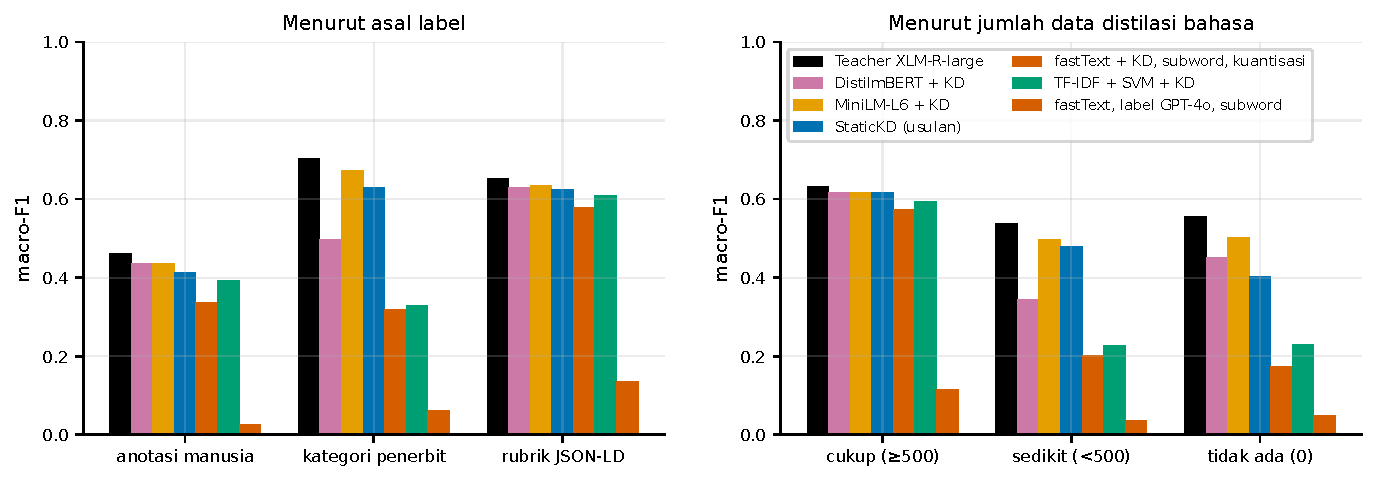
\includegraphics[width=0.9\textwidth]{figures/fig_groups.pdf}
\caption{Macro-F1 set uji menurut asal label (kiri) dan menurut jumlah data distilasi di bahasa artikel (kanan).}
\label{fig:groups}
\end{figure*}

\subsection{Validitas Label Silver}
\label{sec:res-validity}
Label silver diperiksa secara tidak langsung dengan dua cara.
\begin{enumerate}
  \item \textbf{Perbandingan dengan label manusia di bahasa yang sama.} Seluruh sel bahasa Inggris di set uji terisi sumber berlabel manusia. Karena itu diambil sampel terpisah berisi \val{valid.en.silver.n} artikel CC-NEWS berbahasa Inggris berlabel rubrik JSON-LD dari \val{valid.en.silver.sites} situs yang tidak masuk set uji, maksimal 50 per label.
  \begin{itemize}
    \item Akurasi \eng{teacher} pada label silver adalah \val{valid.en.silver.acc} (macro-F1 \val{valid.en.silver.macro}), sedangkan pada label manusia MN-DS/MasakhaNEWS \val{valid.en.human.acc} (macro-F1 \val{valid.en.human.macro}).
    \item Akurasinya lebih tinggi pada label silver di \val{valid.en.labels_higher} dari 17 label (Wilcoxon $p$ \val{valid.en.wilcoxon.p}).
    \item Urutan tingkat kesulitan label pada kedua jenis label berkorelasi ($\rho=\val{valid.en.label_rho}$, $p$ \val{valid.en.label_rho.p}).
  \end{itemize}
  Dengan kata lain, label silver tidak lebih bising daripada label manusia yang tersedia, setidaknya jika diukur dengan kesepakatan terhadap \eng{teacher}. Label yang sulit (\eng{society}, \eng{human interest}, \eng{religion}) sulit di kedua jenis label.
  \item \textbf{Pemeriksaan per kategori sumber}, hanya pada bahasa yang tercakup pra-latih XLM-R. Median kesepakatan \eng{teacher} dengan label hasil pemetaan per kategori adalah \val{mapcheck.masakhanews.median} untuk MasakhaNEWS, \val{mapcheck.mnds.median} untuk MN-DS, \val{mapcheck.l3cube_indic.median} untuk L3Cube, dan \val{mapcheck.ccnews_jsonld.median} untuk rubrik CC-NEWS. Kesepakatan terendah muncul pada dua jenis kategori.
  \begin{itemize}
    \item Kategori sumber yang cakupannya lebih luas daripada topik IPTC tujuannya. Contohnya, MasakhaNEWS \eng{politics} hanya \val{mapcheck.masakha_politics} sesuai, dengan alternatif utama \val{mapcheck.masakha_politics.alt}.
    \item Label yang batasnya kabur bahkan bagi anotator manusia, misalnya MN-DS \eng{society}, sejalan dengan kesepakatan antaranotator yang rendah pada label tersebut~\cite{kuzman2025llm}.
  \end{itemize}
\end{enumerate}
Karena itu, skor absolut pada label berskema non-IPTC merupakan batas bawah akurasi yang sebenarnya, sedangkan perbandingan antarmodel tetap sahih karena semua model dinilai terhadap label yang sama.

\subsection{Ablasi, \eng{Temperature}, dan \eng{Ensemble} (RQ3)}
\TabAblation
\TabAblationGroups
Tabel~\ref{tab:ablation} merangkum kontribusi setiap komponen, dengan lima \eng{seed} per varian.
\begin{itemize}
  \item \textbf{Data distilasi multibahasa adalah komponen terpenting.} Distilasi hanya pada EMMediaTopic (4 bahasa) menurunkan macro-F1 uji sebesar \val{abl.emm_only.test_macro.delta} dan kesepakatan \eng{held-out} sebesar \val{abl.emm_only.heldout_acc.delta}.
  \item \textbf{Inisialisasi embedding yang selaras lintas bahasa.} Inisialisasi acak mengubah macro-F1 uji sebesar \val{abl.random_init.test_macro.delta} ($p$ \val{abl.random_init.test_macro.p}).
  \item \textbf{\eng{Fine-tuning} embedding: kecocokan in-distribusi vs transfer.} Membekukan embedding potion dan hanya melatih kepala linear menurunkan dev sebesar \val{abl.frozen.dev_macro.delta} ($p$ \val{abl.frozen.dev_macro.p}) dan kesepakatan \eng{held-out} sebesar \val{abl.frozen.heldout_acc.delta} ($p$ \val{abl.frozen.heldout_acc.p}), tetapi \emph{menaikkan} macro-F1 uji sebesar \val{abl.frozen.test_macro.delta} ($p$ \val{abl.frozen.test_macro.p}). Tabel~\ref{tab:ablation-groups} menunjukkan bahwa kenaikan ini seluruhnya berasal dari bahasa dengan sedikit data distilasi (\val{ablgrp.frozen.sedikit.delta}) dan tanpa data distilasi (\val{ablgrp.frozen.tidakada.delta}), sedangkan di bahasa kaya data embedding beku lebih lemah (\val{ablgrp.frozen.cukup.delta}).
  \item \textbf{\eng{Soft label}.} Label keras \eng{teacher} mengubah macro-F1 uji sebesar \val{abl.hard.test_macro.delta} ($p$ \val{abl.hard.test_macro.p}) dan dev sebesar \val{abl.hard.dev_macro.delta} ($p$ \val{abl.hard.dev_macro.p}).
  \item \textbf{Ukuran data.} Mengurangi data ke 130 ribu dokumen mengubah macro-F1 uji sebesar \val{abl.data130k.test_macro.delta} ($p$ \val{abl.data130k.test_macro.p}).
  \item \textbf{\eng{Token dropout}.} Tanpa \eng{token dropout}, macro-F1 uji berubah sebesar \val{abl.no_tdrop.test_macro.delta} ($p$ \val{abl.no_tdrop.test_macro.p}).
  \item \textbf{Kepala MLP.} Kepala MLP, yang tidak dapat dilipat, mengubah macro-F1 uji sebesar \val{abl.mlp.test_macro.delta} ($p$ \val{abl.mlp.test_macro.p}).
\end{itemize}

\textbf{\eng{Temperature}} (Gbr.~\ref{fig:temperature}). Dibanding $\tau=1$:
\begin{itemize}
  \item $\tau=2$, nilai yang lazim dipakai~\cite{hinton2015distilling}, mengubah dev sebesar \val{abl.tau2.dev_macro.delta} ($p$ \val{abl.tau2.dev_macro.p}) dan kesepakatan \eng{held-out} sebesar \val{abl.tau2.heldout_acc.delta} ($p$ \val{abl.tau2.heldout_acc.p});
  \item $\tau=4$ mengubah macro-F1 uji sebesar \val{abl.tau4.test_macro.delta} ($p$ \val{abl.tau4.test_macro.p}).
\end{itemize}

\textbf{Varian eksplorasi} (bigram \eng{hashing}, \eng{pooling} idf, bobot keyakinan, label GPT-4o) tidak memperbaiki set uji. Hasilnya: bigram \val{abl.bigram.test_macro.delta}, idf \val{abl.idf.test_macro.delta}, bobot keyakinan \val{abl.conf.test_macro.delta}, dan CE GPT-4o \val{abl.gpt_ce.test_macro.delta}.

\textbf{\eng{Ensemble}} (Gbr.~\ref{fig:ensemble}). Menaikkan ukuran \eng{ensemble} dari satu ke tiga \eng{seed} mengubah macro-F1 uji rata-rata dari \val{ens.k1.test_macro} menjadi \val{ens.k3.test_macro}, dan kesepakatan \eng{held-out} dari \val{ens.k1.heldout_acc} menjadi \val{ens.k3.heldout_acc}. Sepuluh \eng{seed} memberi \val{ens.k10.test_macro}. Semua ukuran \eng{ensemble} tetap berupa satu tabel dengan biaya inferensi yang sama.

\begin{figure*}[!t]
\centering
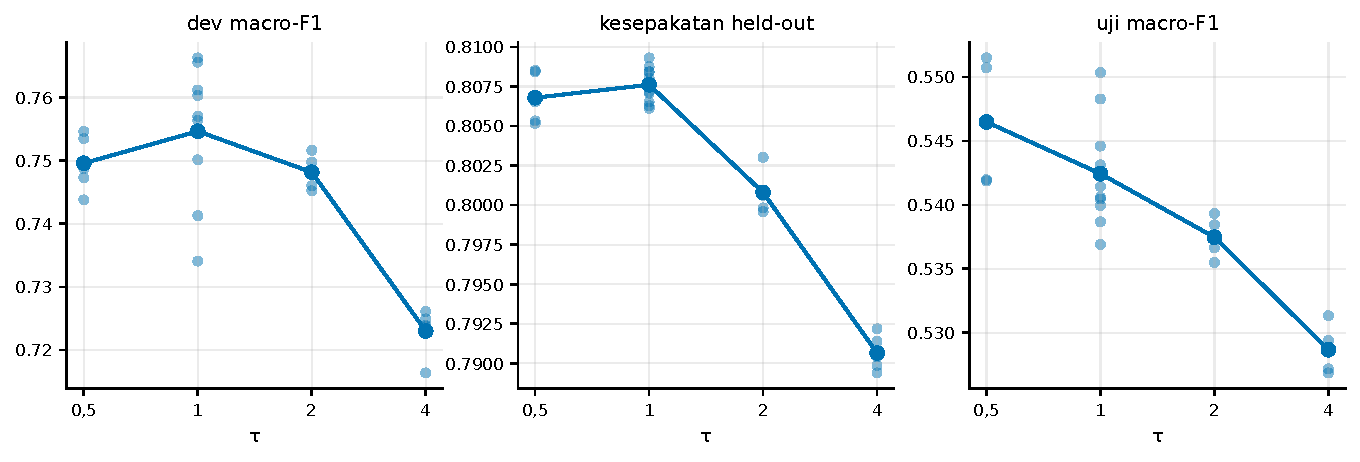
\includegraphics[width=0.9\textwidth]{figures/fig_temperature.pdf}
\caption{Pengaruh \eng{temperature} distilasi. Titik = satu \eng{seed}, garis = rata-rata.}
\label{fig:temperature}
\end{figure*}

\begin{figure}[!t]
\centering
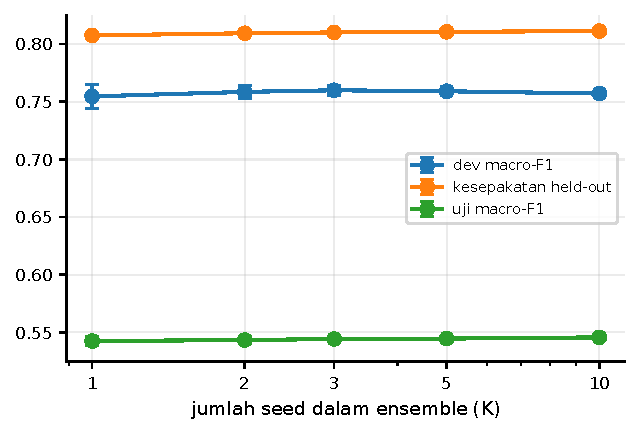
\includegraphics[width=0.85\columnwidth]{figures/fig_ensemble_size.pdf}
\caption{Pengaruh ukuran \eng{ensemble} tabel (rata-rata $\pm$ SD atas kombinasi \eng{seed}).}
\label{fig:ensemble}
\end{figure}

\subsection{Efisiensi CPU (RQ1)}
\label{sec:res-eff}
\TabEff
Tabel~\ref{tab:eff} dan Gbr.~\ref{fig:tradeoff}--\ref{fig:latency} menunjukkan efisiensi seluruh model.

\textbf{\eng{Teacher}.} Dalam PyTorch fp32, \eng{teacher} membutuhkan \val{eff.teacher.latency_ms_p50_1c}~ms per artikel pada satu \eng{core}, dengan \eng{throughput} \val{eff.teacher.docs_per_sec_1c} artikel per detik. Konfigurasi CPU terbaiknya, ONNX int8, membutuhkan \val{eff.teacher_onnx_int8.latency_ms_p50_1c}~ms dengan \eng{throughput} \val{eff.teacher_onnx_int8.docs_per_sec_1c} artikel per detik. Untuk satu juta artikel per hari dibutuhkan \val{eff.teacher_onnx_int8.cores1M} \eng{core} (ONNX int8) sampai \val{eff.teacher.cores1M} \eng{core} (PyTorch) khusus untuk klasifikasi.

\textbf{StaticKD.}
\begin{itemize}
  \item Latensi \val{eff.statickd.latency_ms_p50_1c}~ms dan \eng{throughput} \val{eff.statickd.docs_per_sec_1c} artikel per detik per \eng{core}.
  \item Sekitar \val{eff.statickd.speedup_onnx} kali lebih cepat dari \eng{teacher} ONNX int8, \val{eff.statickd.speedup_pt} kali lebih cepat dari \eng{teacher} PyTorch, dan \val{eff.speed_vs_minilm} kali lebih cepat dari MiniLM-L6.
  \item Ukuran file \val{eff.size_ratio_onnx} kali lebih kecil dari \eng{teacher} ONNX int8.
  \item Satu juta artikel per hari hanya membutuhkan \val{eff.statickd.cores1M} \eng{core}.
  \item RAM model \val{eff.statickd.ram}~MB, sebagian besar dipakai struktur tokenizer. Varian \eng{compact} menurunkannya ke \val{eff.statickd_compact.ram}~MB.
  \item \textbf{Tokenisasi adalah hampir seluruh biaya.} Pada satu \eng{thread}, tokenisasi (rata-rata \val{prof.statickd.tokens} token per artikel) memakan \val{prof.statickd.tokshare} waktu prediksi. \eng{Pooling} tabel sendiri berjalan pada \val{prof.statickd.pool_dps} artikel per detik. Batas kecepatan StaticKD karena itu ditentukan oleh implementasi tokenizer, bukan oleh model.
\end{itemize}

\begin{figure}[!t]
\centering
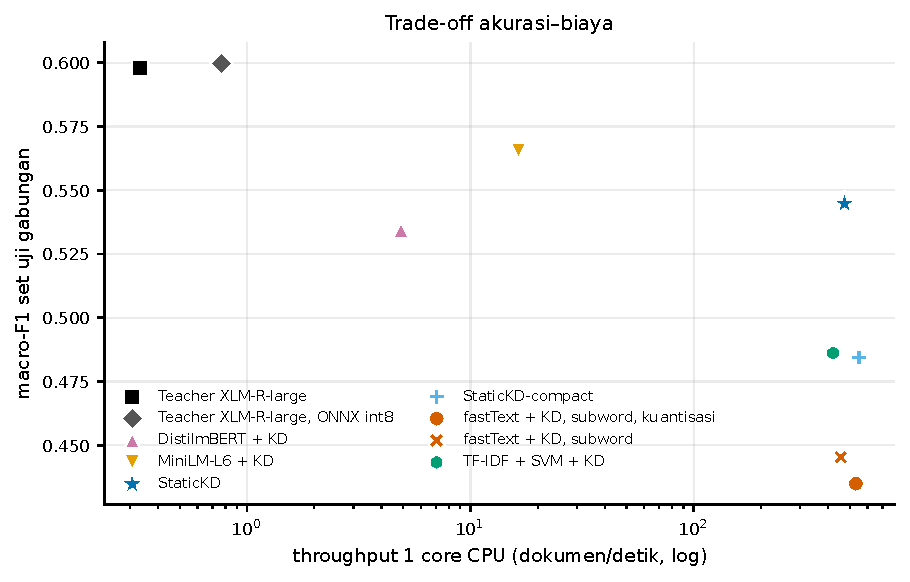
\includegraphics[width=\columnwidth]{figures/fig_tradeoff.pdf}
\caption{\eng{Trade-off} macro-F1 set uji gabungan terhadap \eng{throughput} satu \eng{core} CPU (skala log).}
\label{fig:tradeoff}
\end{figure}

\begin{figure*}[!t]
\centering
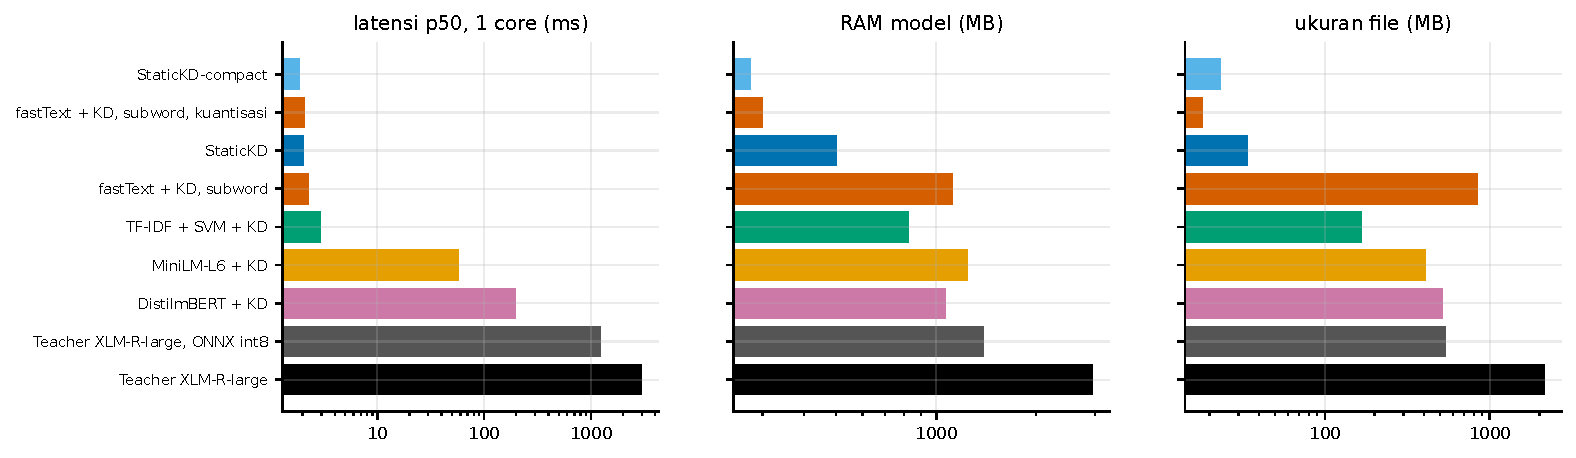
\includegraphics[width=0.9\textwidth]{figures/fig_latency_ram_size.pdf}
\caption{Latensi per artikel, RAM model, dan ukuran file (skala log).}
\label{fig:latency}
\end{figure*}

\subsection{Analisis per Bahasa dan per Label (RQ4)}
\TabFactors

\textbf{Per bahasa} (Gbr.~\ref{fig:lang}).
\begin{itemize}
  \item Median selisih akurasi StaticKD terhadap \eng{teacher} per bahasa uji adalah \val{lang.gap.median}. StaticKD lebih akurat daripada fastText + KD di \val{lang.static_better_ft} dari \val{lang.n} bahasa.
  \item Di \eng{held-out} (\val{fac.langs} bahasa dengan minimal 20 dokumen), kesepakatan StaticKD berkorelasi dengan log jumlah data distilasi ($\rho=\val{fac.data.rho}$, $p$ \val{fac.data.p}) dan dengan keyakinan \eng{teacher} ($\rho=\val{fac.conf.rho}$, $p$ \val{fac.conf.p}), tetapi tidak berbeda antarsistem tulisan (Kruskal--Wallis $H=\val{fac.kw.H}$, $p$ \val{fac.kw.p}) (Tabel~\ref{tab:factors}).
  \item \textbf{Bahasa yang lemah.} Akurasi StaticKD rata-rata \val{lang.outxlmr.static_acc} (\eng{teacher} \val{lang.outxlmr.teacher_acc}) pada bahasa di luar pra-latih XLM-R (\val{lang.outxlmr.langs}), yang juga tidak ada di data distilasi.
  \item \textbf{Cakupan token.} Pada \val{lang.vlowcov.n} bahasa (\val{lang.vlowcov.langs}), kurang dari separuh kemunculan token pernah muncul minimal 10 kali di data distilasi (maksimal \val{lang.vlowcov.cov_max}). Meski begitu, StaticKD tetap mencapai akurasi rata-rata \val{lang.vlowcov.static_acc} (\eng{teacher} \val{lang.vlowcov.teacher_acc}). Varian \eng{compact} membuang token-token tersebut dari tokenizer, dan akurasinya di bahasa-bahasa ini jatuh ke \val{lang.vlowcov.compact_acc}. Di bahasa lainnya, akurasi \eng{compact} \val{lang.restcov.compact_acc} dibanding \val{lang.restcov.static_acc} untuk StaticKD penuh. Bagian~\ref{sec:discussion} membahas mekanisme di balik pola ini.
\end{itemize}

\begin{figure*}[!t]
\centering
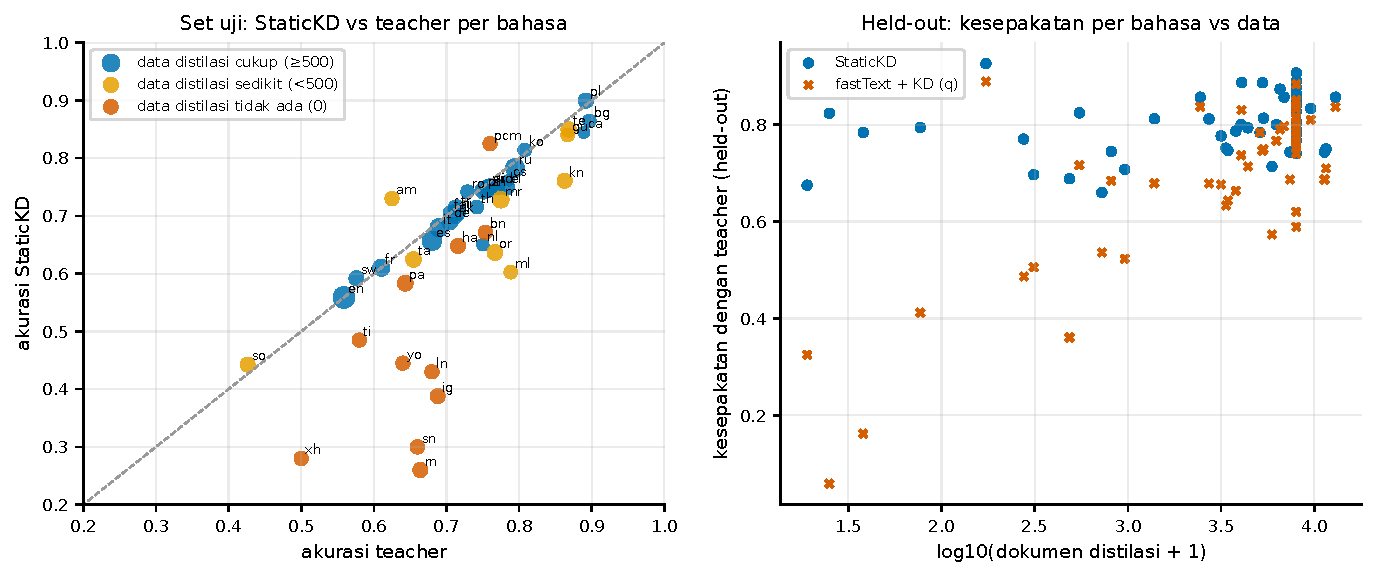
\includegraphics[width=0.9\textwidth]{figures/fig_per_language.pdf}
\caption{Kiri: akurasi StaticKD terhadap akurasi \eng{teacher} per bahasa uji (warna = jumlah data distilasi bahasa, ukuran = jumlah artikel). Kanan: kesepakatan per bahasa \eng{held-out} terhadap jumlah data distilasi, StaticKD vs fastText + KD.}
\label{fig:lang}
\end{figure*}

\textbf{Per label} (Gbr.~\ref{fig:label}).
\begin{itemize}
  \item Label tersulit bagi StaticKD adalah \val{label.hardest}, sedangkan yang termudah \val{label.easiest}.
  \item Selisih terbesar terhadap \eng{teacher} ada pada \val{label.biggest_gap}.
  \item Kebingungan terbesar adalah \val{label.top_confusions}.
\end{itemize}

\begin{figure*}[!t]
\centering
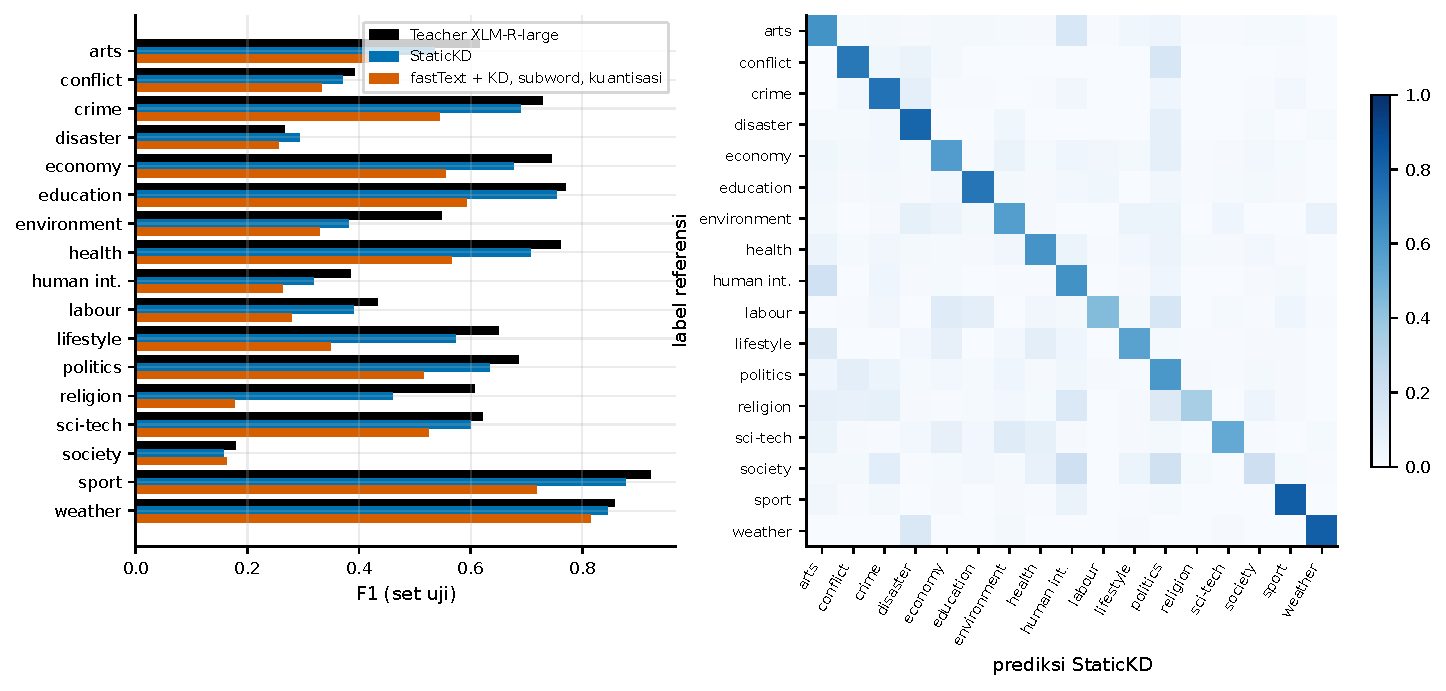
\includegraphics[width=0.9\textwidth]{figures/fig_per_label.pdf}
\caption{F1 per label di set uji (kiri) dan \eng{confusion matrix} StaticKD yang dinormalisasi per label referensi (kanan).}
\label{fig:label}
\end{figure*}

\subsection{Kalibrasi dan Mode \eng{Cascade}}
\TabCascade
\textbf{Kalibrasi.} ECE StaticKD adalah \val{ece.statickd.dev} di dev dan \val{ece.statickd.test} di set uji, lebih rendah daripada ECE \eng{teacher} (\val{ece.teacher.dev} dan \val{ece.teacher.test}). Kedua model menjadi terlalu yakin (\eng{overconfident}) di set uji yang berada di luar distribusi latih (Gbr.~\ref{fig:calib}).

\textbf{\eng{Cascade}.} Artikel dengan keyakinan StaticKD minimal $\theta$ diputuskan oleh StaticKD, dan sisanya dikirim ke \eng{teacher} (Tabel~\ref{tab:cascade}). Dengan $\theta=0{,}8$:
\begin{itemize}
  \item StaticKD memutuskan \val{casc.08.coverage} artikel dengan akurasi \val{casc.08.acc_covered};
  \item akurasi \eng{cascade} keseluruhan menjadi \val{casc.08.accuracy} (\eng{teacher} saja: \val{casc.101.accuracy}) dan macro-F1 \val{casc.08.macro_f1} (\eng{teacher} saja: \val{casc.101.macro_f1});
  \item \eng{throughput} efektifnya \val{casc.08.docs_per_sec} artikel per detik per \eng{core}, dibanding \val{casc.101.docs_per_sec} untuk \eng{teacher} saja.
\end{itemize}
Jadi dengan hanya sekitar dua perlima artikel yang dikirim ke \eng{teacher}, \eng{cascade} menyamai akurasi \eng{teacher}.

\begin{figure}[!t]
\centering
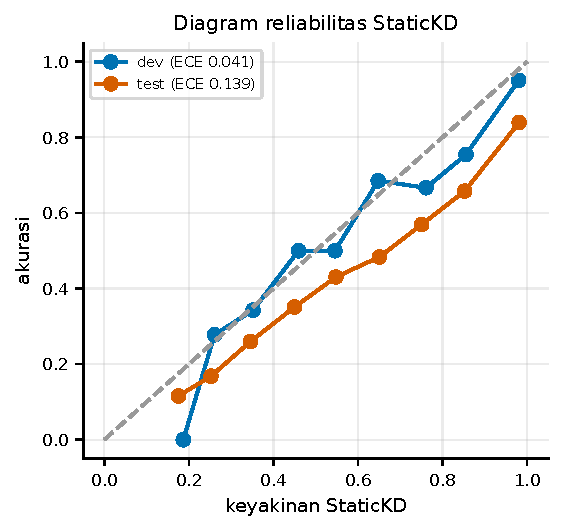
\includegraphics[width=0.8\columnwidth]{figures/fig_calibration.pdf}
\caption{Diagram reliabilitas StaticKD pada dev dan set uji.}
\label{fig:calib}
\end{figure}
